\documentclass{../pl-slide}

\usepackage[british]{babel}
\usepackage[british]{datetime2}
\usepackage{ulem}
\usepackage{qrcode}

\usepackage{tikz,calc}
\usetikzlibrary{shapes, shapes, arrows, chains, fit, quotes}

\tikzstyle{discoverydiagramnode} = [rectangle, rounded corners, minimum width=3cm, minimum height=1cm,text centered, draw=white]
\tikzstyle{trienode} = [draw=text-color, rounded corners]
\tikzstyle{bucket} = [draw=text-color, rectangle]

\usepackage{pgf-umlsd}

\definecolor{verystable}{HTML}{13f6e9}
\definecolor{stableenough}{HTML}{ccff00}
\definecolor{unstable}{HTML}{ffa500}

\settheme{ipfs-thing-2023}

%Information to be included in the title page:
\title{Effectiveness of Bitswap Discovery Process }
\author{Gui Michel}
\avatar{../resources/avatar.jpg}
\handle{@guissou}
\group{Probelab}
\institute{Protocol Labs}
\event{IPFS Thing}
\date{\DTMdate{2023-04-15}}

\begin{document}

\frame{\titlepage}

\begin{frame}
\frametitle{Motivation}
\begin{itemize}
        \itemc Measure Bitswap content discovery efficiency
        \itemc Evaluate Bitswap \texttt{ProviderSearchDelay} magic value set to 1 second
        \itemc Optimize content routing efficiency

\end{itemize}
\end{frame}

\begin{frame}
\frametitle{Bitswap Discovery Process}

\begin{enumerate}
	\item \texttt{go-bitswap} broadcasts a \texttt{WANT-HAVE} request to directly all connected peers
	\item If the content is found, request is done
	\item If after \texttt{1s} no positive answer is return from the broadcast, start a DHT lookup
	\item When a Provider is found in the DHT, \texttt{go-bitswap} sends a \texttt{WANT-BLOCK} request
\end{enumerate}

\end{frame}

\begin{frame}
\frametitle{Measurements Setup}
\begin{itemize}
        \itemc Request CIDs collected by sniffing the Bitswap network
        \itemc Bitswap has 15 seconds to find and fetch 1 block
        \itemc Prevent DHT lookup inside Bitswap
        \itemc If Bitswap fails to discover content, verify if content is still available
        \itemc Prevent recursive content resolution
        \itemc Ran on a Google Cloud VM in Central Europe in Dec. 2022
\end{itemize}
\end{frame}

\begin{frame}
\frametitle{Discovery Process Stats}
\begin{itemize}
        \itemc \texttt{98.37\%} discovery success rate (within 15 seconds)
        \itemc On average \texttt{856} distinct remote peers are solicited for each Bitswap request
        \itemc On average \texttt{1714} messages are sent for each Bitswap request
\end{itemize}
\end{frame}

\begin{frame}
\frametitle{Content Providers Stats}
\greencube\hspace{0.4em} Total requests: 50'062
\begin{columns}[onlytextwidth]
\begin{column}{0.35\textwidth}
    \begin{center}
                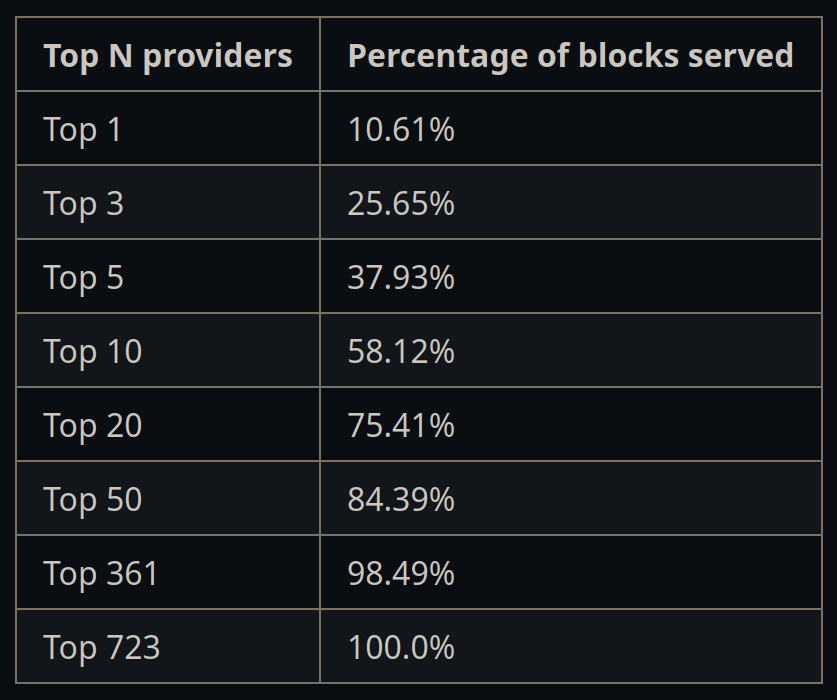
\includegraphics[width=\textwidth]{plots/top_provs.png}
    \end{center}
\end{column}
\begin{column}{0.64\textwidth}
    \begin{center}
                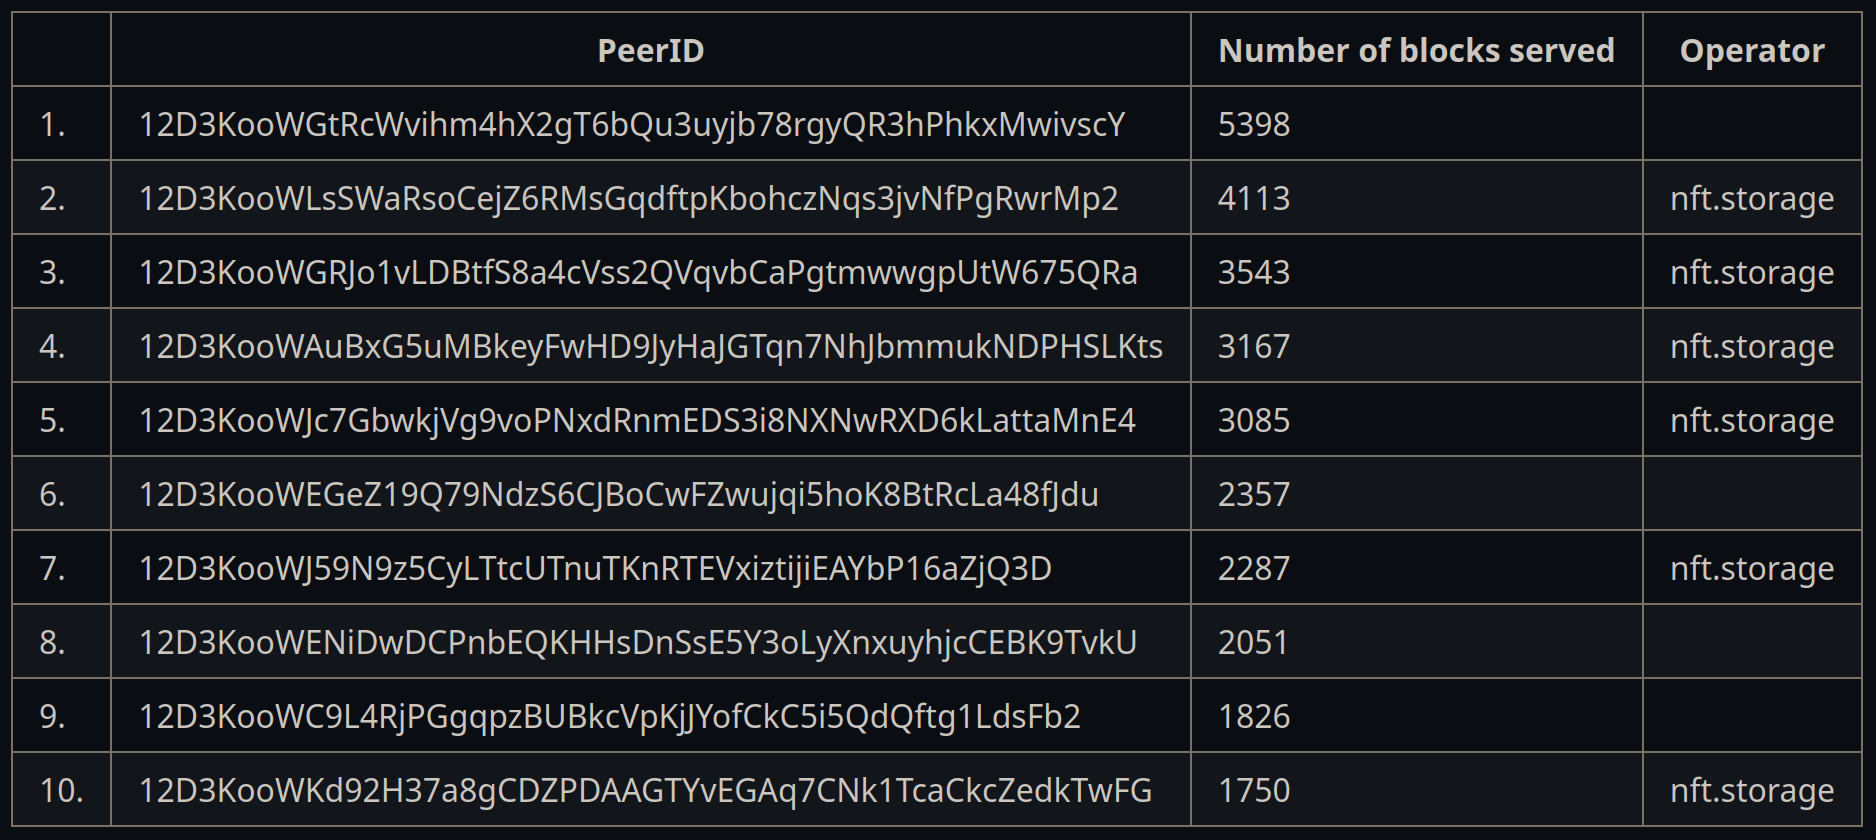
\includegraphics[width=\textwidth]{plots/top10.png}
    \end{center}
\end{column}
\end{columns}
\end{frame}

\begin{frame}
\frametitle{Bitswap Discovery + Fetch Latencies}
\begin{columns}[onlytextwidth]
\begin{column}{0.49\textwidth}
    \begin{center}
                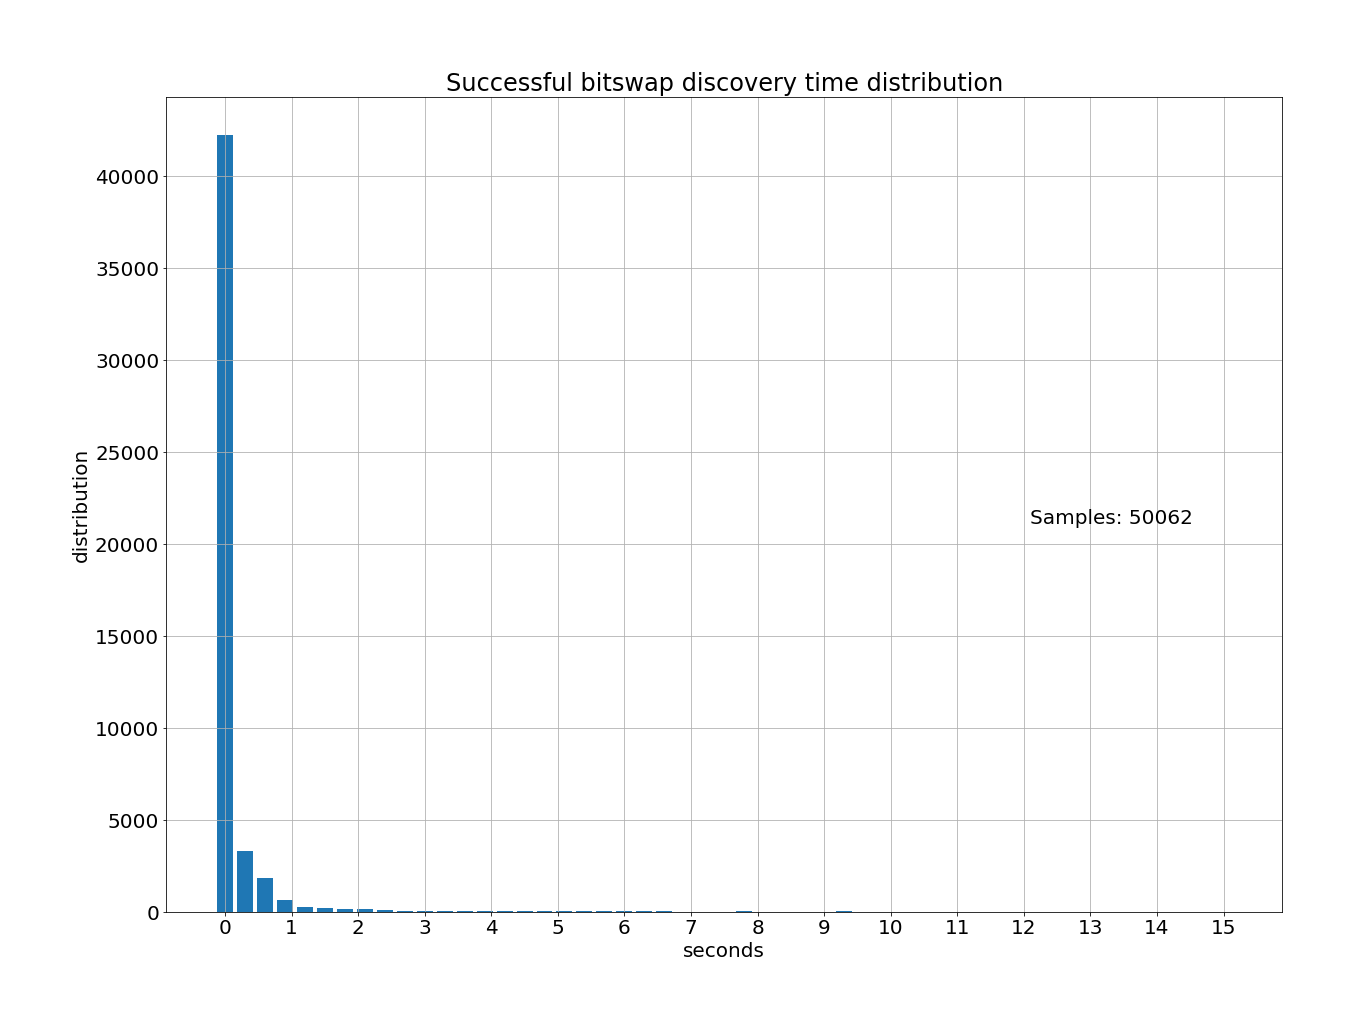
\includegraphics[width=\textwidth]{plots/pdf15.png}
    \end{center}
\end{column}
\begin{column}{0.49\textwidth}
    \begin{center}
                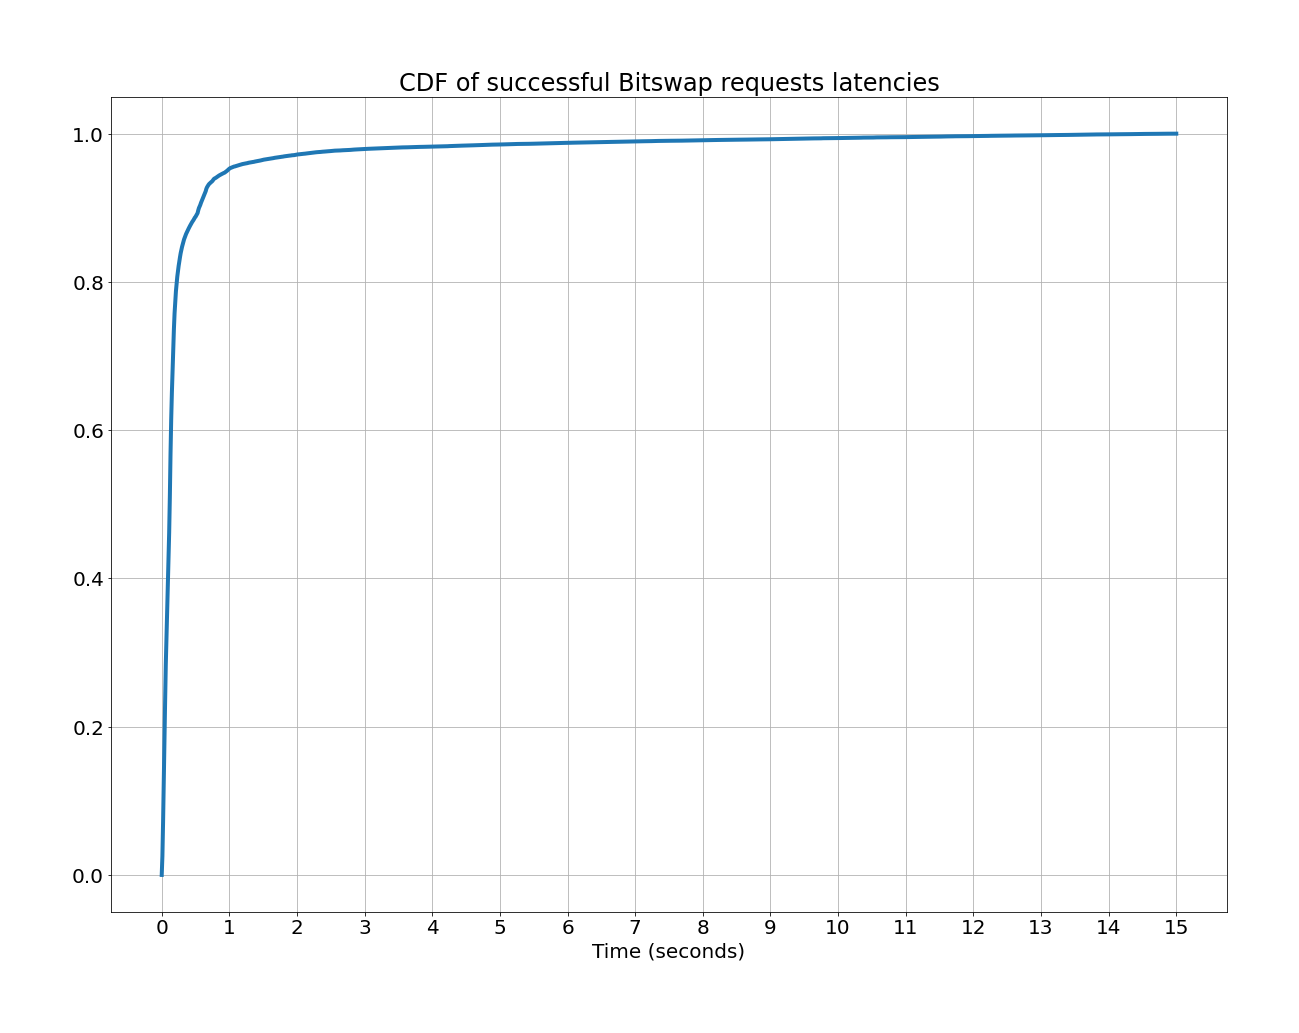
\includegraphics[width=\textwidth]{plots/cdf15.png}
    \end{center}
\end{column}
\end{columns}

\end{frame}

\begin{frame}
\frametitle{Bitswap Discovery + Fetch Latencies Zoom}
\begin{columns}[onlytextwidth]
\begin{column}{0.49\textwidth}
    \begin{center}
                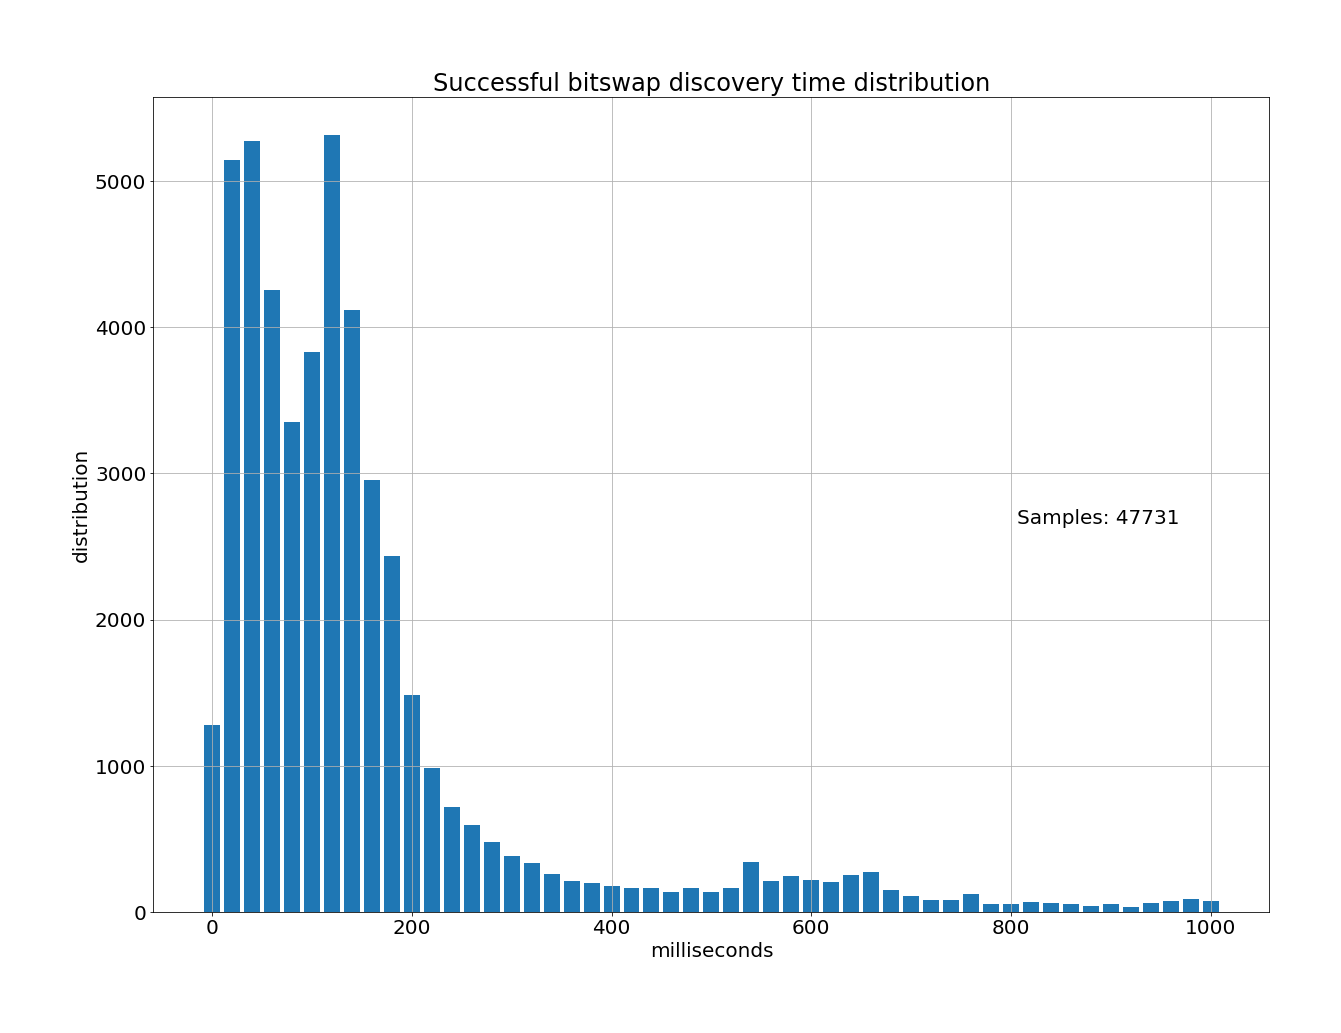
\includegraphics[width=\textwidth]{plots/pdf1.png}
    \end{center}
\end{column}
\begin{column}{0.49\textwidth}
    \begin{center}
                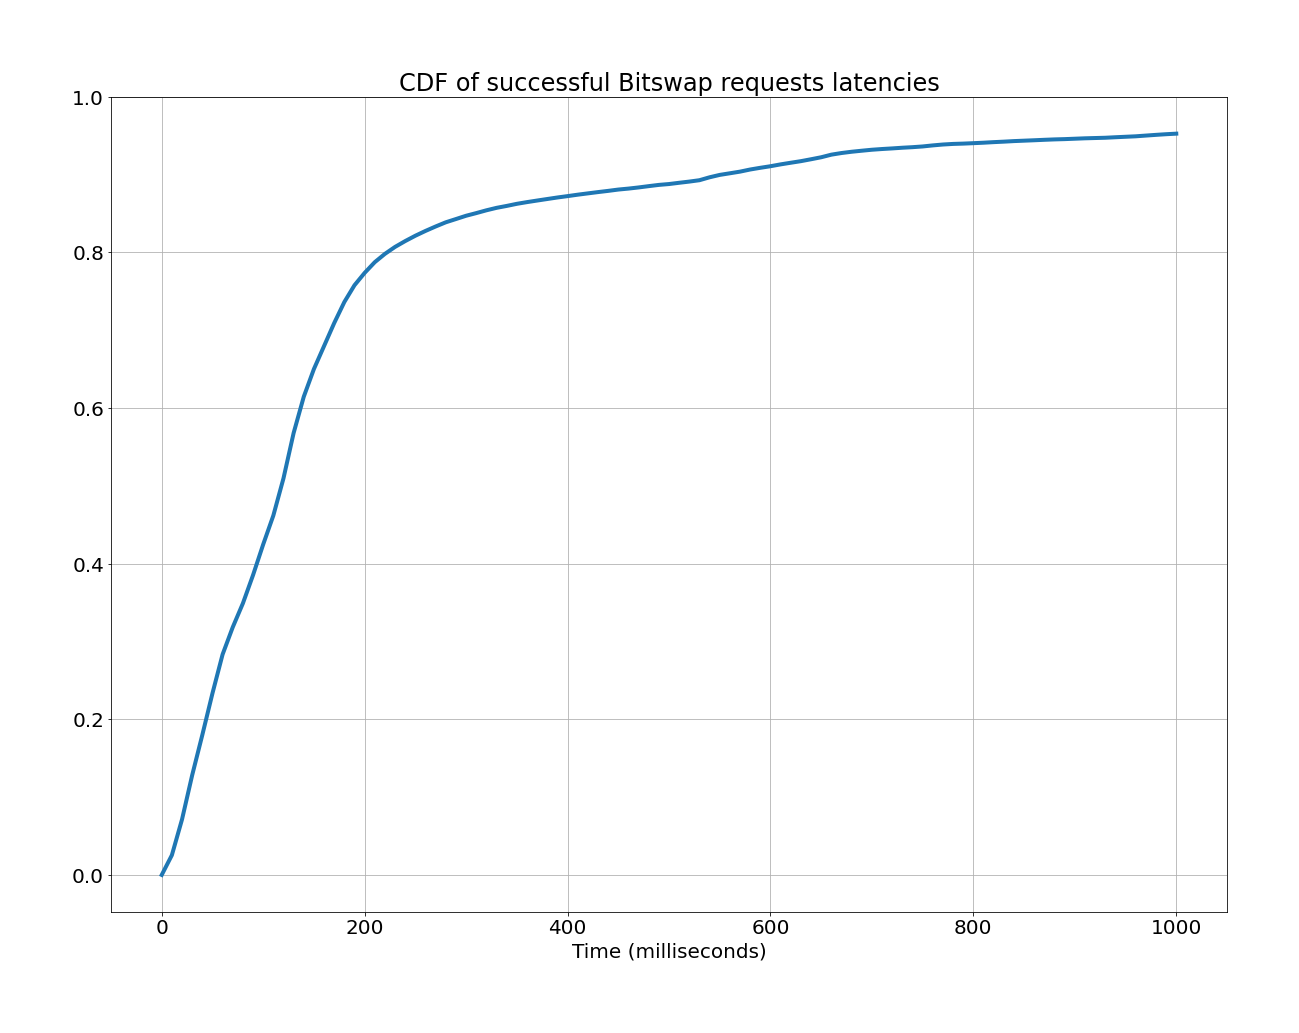
\includegraphics[width=\textwidth]{plots/cdf1.png}
    \end{center}
\end{column}
\end{columns}
\end{frame}

\begin{frame}
\frametitle{Recent Developments}

\begin{itemize}
	\itemc Connection manager now limits to \texttt{32/96} inbound connections (\href{https://github.com/ipfs/kubo/pull/9483}{\texttt{ipfs/kubo\#9483}})
	\itemc Worse TTFB when \texttt{ProviderSearchDelay} is set to \texttt{0} (\href{https://github.com/ipfs/kubo/issues/8807}{\texttt{ipfs/kubo\#8807}})
	\itemc Certainly caused by side effects/bugs in \texttt{go-bitswap} (\href{https://github.com/ipfs/kubo/pull/9530}{\texttt{ipfs/kubo\#9530}})
\end{itemize}
\end{frame}

\begin{frame}
\frametitle{Takeaways}
\begin{itemize}
        \itemc Bitswap is currently \textbf{fast} (discovery+fetch $\leq 200$ms in $80\%$) and \textbf{accurate} ($98.37\%$ of accessible content found)
        \itemc Bitswap is \textbf{inefficient} ($856$ peers solicited for each request)
        \itemc Bitswap content discovery \textbf{does NOT scale} (e.g if the network grows by 10x, the number of open connection must be 10x to keep the same discovery success rate)
        \itemc The top 20 peers serve $75\%$ of the requested content
        \bigskip
        \itemc Data transfer and content routing should probably NOT be bundled together
\end{itemize}
\end{frame}

\begin{frame}
\frametitle{References}
\begin{columns}[onlytextwidth]
\begin{column}{0.60\textwidth}
\begin{itemize}
        \itemc Complete measurement methodology
        \itemc Additional data and plots
        \itemc Improvement recommendations
\end{itemize}
\end{column}
\begin{column}{0.38\textwidth}
\begin{center}
\qrcode[height=4cm]{https://github.com/protocol/network-measurements/blob/master/results/rfm16-bitswap-discovery-effectiveness.md}\\
\medskip
RFM-16 Report
\bigskip
\end{center}
\end{column}
\end{columns}

\end{frame}


\end{document}